\documentclass[12pt]{article}

\usepackage[margin=1in]{geometry}
\usepackage{amsmath,amsthm,amssymb}
\usepackage{mathrsfs}
\usepackage{mathtools}
\usepackage{enumitem}
\usepackage{physics}
\usepackage{pdfpages}

\newcommand{\magsq}[1]{\big|#1\big|^2}
\newcommand{\avg}[1]{\left<#1\right>}

\begin{document}
	
\title{Homework 5}
\author{Sean Ericson \\ Phys 684}
\maketitle

\section*{Problem 1}
We start with the Maxwell wave equation
\[ \left(\vec{\nabla}^2-\frac{1}{c^2}\pdv[2]{t}\right)\vec{E}(\vec{r},t) = \mu_0\pdv[2]{t}\vec{P}(\vec{r}, t), \]
where
\[ \vec{E}(\vec{r},t) = \vec{E}_+(z,t) + \vec{E}_-(z,t); \quad \vec{E}_\pm(z,t) = \frac{1}{2}\hat{x}E_0(z,t)e^{\mp i\alpha(z,t)}, \]
\[ \vec{P}(\vec{r},t) = \vec{P}_+(z,t) + \vec{P}_-(z,t) = \frac{1}{2}\hat{x}\left(P_0(z,t)e^{-i\alpha(z,t)} + \text{c.c}\right), \]
\[ \alpha(z,t) = \omega t - kz - \phi(z,t), \]
and $E_0(z,t)\in\mathbb{R}$ while $P_0(z,t)\in\mathbb{C}$.
Next, we note that
\begin{align*}
    2\pdv{z}\abs{E_\pm} &= \left(E_0' \mp iE_0\alpha'\right)e^{\mp i\alpha}, \\
    2\pdv{t}\abs{E_\pm} &= \left(\dot{E}_0 \mp iE_0\dot\alpha\right)e^{\mp i\alpha}, \\
    2\pdv{t}\abs{P_\pm} &= \left(\dot{P}_0 \mp P_0\dot\alpha\right)e^{\mp i\alpha}
\end{align*}

\section*{Problem 2}
Starting with
\begin{align*}
    \dot{\tilde{\rho}}_{21} &= -\gamma \tilde{\rho}_{21} - i\delta\tilde{\rho}_{21} + i \frac{\Omega_0}{2}\left(\rho_{22}-\rho_{11}\right) \\
    \dot{\rho}_{22} &= -\gamma_2\rho_{22} + \Re[i\Omega_0^*\tilde{\rho}_{21}],
\end{align*}
we first drop the tildes, then let $\rho_{21} = \frac{1}{2}(u - iv)$, and $\Omega_0 = \Omega_0' + i\Omega_0''$. Plugging these in, we get
\begin{alignat*}{3}
    &\quad & \frac{1}{2}(\dot{u} - i\dot{v}) &= -\frac{\gamma}{2}(u-iv) - i\frac{\delta}{2}(u-iv) + \frac{i}{2}\left(\Omega_0' + i\Omega_0''\right)\left(2\rho_{22} - 1\right) \\
    &\quad & \dot{\rho}_{22} &= -\gamma_2\rho_{22} + \frac{1}{2}\left(\Omega_0'' u + \Omega_0' v\right) \\
    &\implies\quad & &  \\
    &\quad & \dot{u} &= -\gamma u - \delta v - 2\Omega_0''\rho_{22} + \Omega_0'' \\
    &\quad & \dot{v} &= -\delta u + \gamma v + 2\Omega_0' \rho_{22} - \Omega_0'  \\
    &\quad & \dot{\rho}_{22} &= \frac{\Omega_0''}{2} u + \frac{\Omega_0'}{2}v - \gamma_2\rho_{22}
\end{alignat*}
In the steady state, this is   
\[
\begin{rcases*}
    -\gamma u -\delta v - 2\Omega_0''\rho_{22} = -\Omega_0'' \\
    -\delta u + \gamma v + 2\Omega_0'\rho_{22} = \Omega_0' \\
    \frac{\Omega_0''}{2} u + \frac{\Omega_0'}{2} v - \gamma_2\rho_{22} = 0
\end{rcases*}
\implies
\mqty(-\gamma&-\delta&2\Omega_0''\\-\delta&+\gamma&2\Omega_0'\\\frac{\Omega_0''}{2}&\frac{\Omega_0'}{2}&-\gamma_2)\mqty(u\\v\\\rho_{22}) = \mqty(-\Omega_0''\\\Omega_0\\0)
\]
Inverting and solving, we find
\[ \mqty(\dot{u}\\\dot{v}\\\dot{\rho}_{22}) = \frac{1}{\gamma^2 + \delta^2 + \frac{\gamma}{\gamma_2}\magsq{\Omega_0}}\mqty(\gamma\Omega_0'' - \delta\Omega_0' \\ \delta\Omega_0'' + \gamma\Omega_0' \\ \frac{\gamma\magsq{\Omega_0}}{2\gamma_2}). \]
Or, in terms of just density matrix components,
\begin{align*}
    \tilde{\rho}_{21} &= \frac{-\frac{1}{2}(\delta+i\gamma)\Omega_0}{\gamma^2 + \delta^2 + \frac{\gamma}{\gamma_2}\magsq{\Omega_0}} \\
    \rho_{22} &= \frac{\gamma\magsq{\Omega_0}}{2\gamma_2}\frac{1}{\gamma^2 + \delta^2 + \frac{\gamma}{\gamma_2}\magsq{\Omega_0}} \\
\end{align*}

\section*{Problem 3}
\begin{enumerate}[label=(\alph*)]
    \item 
\end{enumerate}

\section*{Problem 4}
\begin{enumerate}[label=(\alph*)]
    \item 
\end{enumerate}

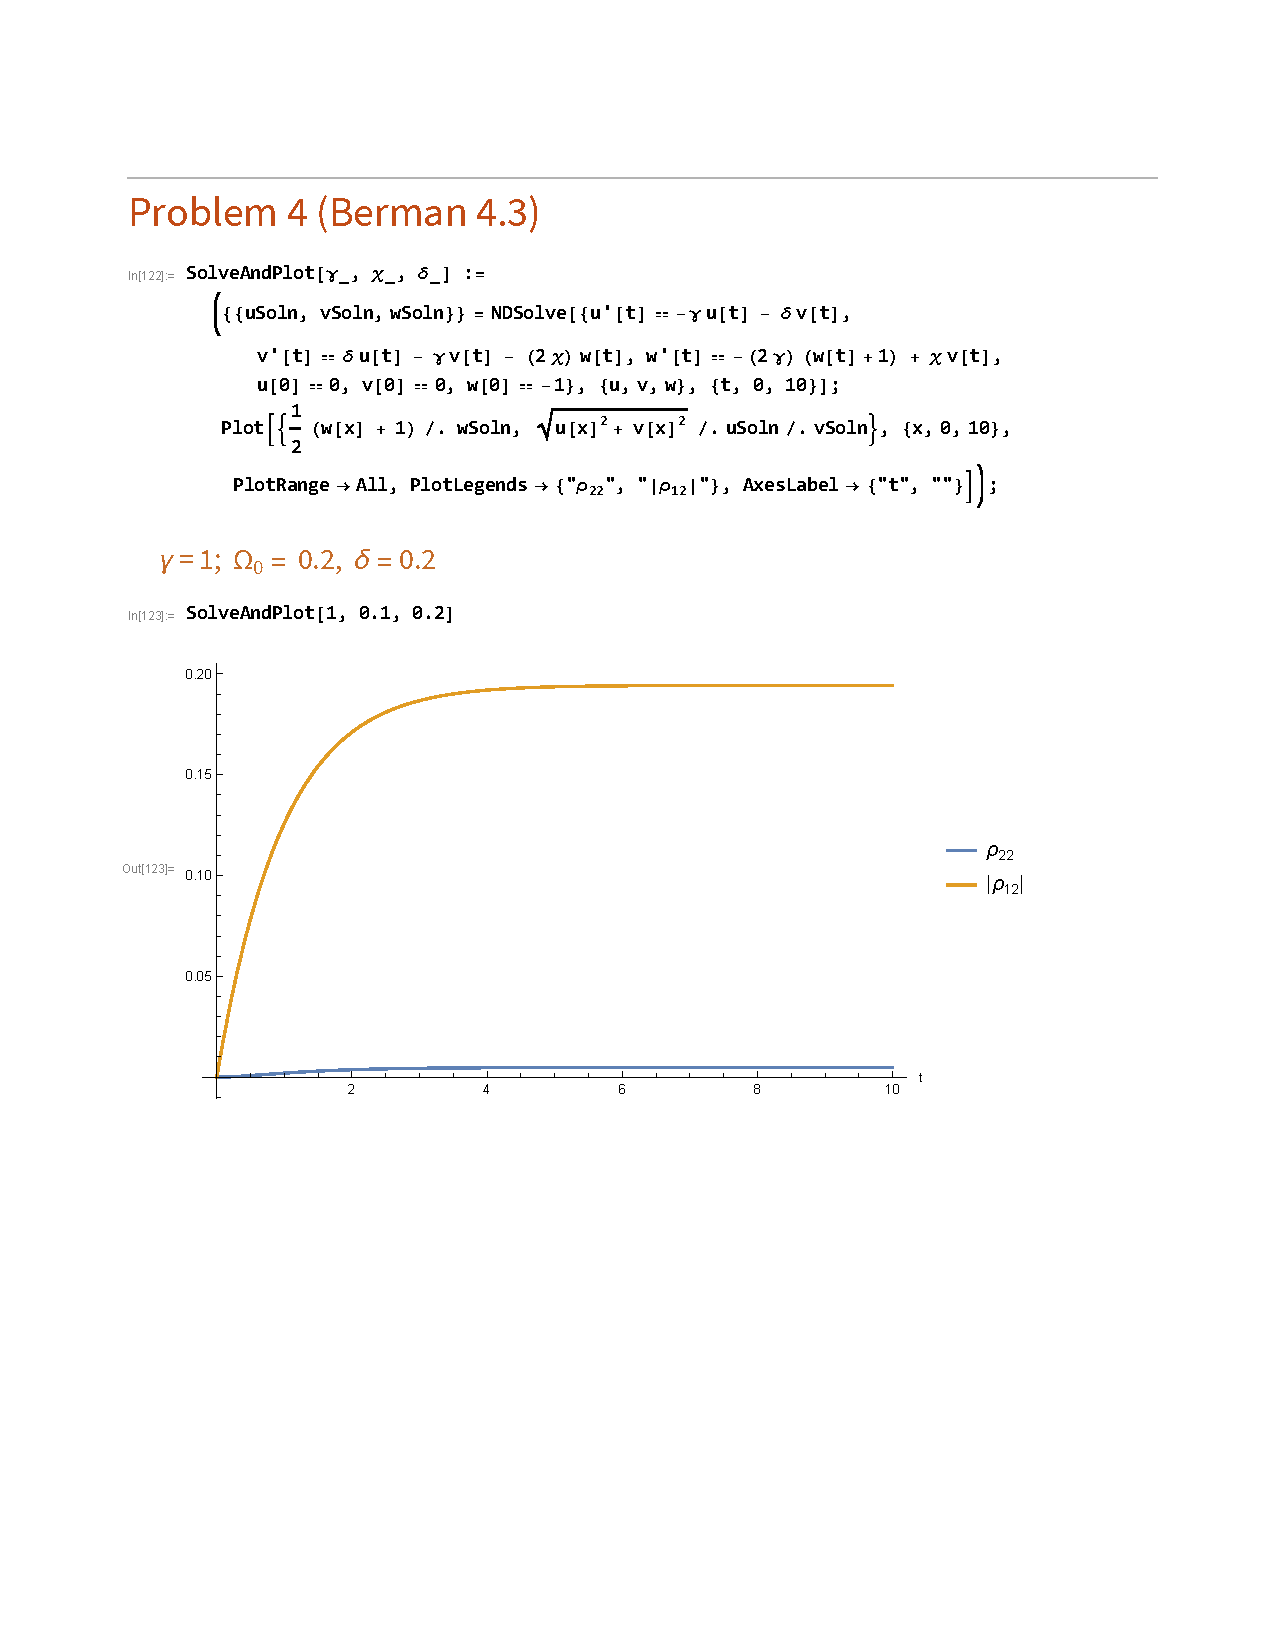
\includepdf[pages=-]{calcs/HW5_mathematica.pdf}
\end{document}